\documentclass[11pt]{article}

\usepackage[margin=1.05in]{geometry}
\usepackage[T1]{fontenc}
\usepackage{lmodern}
\usepackage{microtype}
\usepackage{amsmath,amssymb,amsthm,mathtools}
\usepackage{booktabs}
\usepackage{graphicx}
\usepackage{subcaption}
\usepackage{xcolor}
\usepackage[numbers,sort&compress]{natbib}
\usepackage[colorlinks=true,linkcolor=blue!55!black,citecolor=blue!55!black,urlcolor=blue!55!black]{hyperref}

\graphicspath{{figures/}}

\newtheorem{theorem}{Theorem}
\newtheorem{proposition}{Proposition}
\newtheorem{remark}{Remark}

\DeclareMathOperator{\Cov}{Cov}
\DeclareMathOperator{\Law}{Law}
\DeclareMathOperator{\diag}{diag}

\title{\vspace{-1em}Flow Matching with Stochastic Interpolants:\\
Three Dirac Masses and Gaussian Endpoint Geometry}
\author{}
\date{}

\begin{document}
\maketitle

\begin{abstract}
We study the probability-flow velocity associated with stochastic interpolants
of the form \(X_t=a(t)X_0+b(t)X_1\).  The first case transports a standard
Gaussian source toward a symmetric mixture of three Dirac masses.  In this
semi-discrete setting the density of \(X_t\) is an explicit Gaussian mixture,
so the flow-matching velocity is available as a closed-form conditional
expectation.  Numerical experiments compare linear, variance-preserving, and
cosine schedules and contrast their curved probability-flow trajectories with
the straight rays of semi-discrete optimal transport.  The second case takes
Gaussian endpoints.  We derive the covariance path, the linear velocity field,
and a closed-form flow map for arbitrary schedules \(a,b\).  The terminal map
matches the target covariance but agrees with the Gaussian optimal-transport
map only when the endpoint covariances commute.
\end{abstract}

\section{Introduction}

Flow matching learns deterministic velocity fields whose continuity equation
transports a simple base distribution to a data distribution.  Recent
formulations by \citet{lipman2023flow} and the stochastic-interpolant framework
of \citet{albergo2023stochastic} show that many generative modeling objectives
can be obtained by specifying an interpolation \(X_t\) between two endpoint
random variables and regressing the conditional mean velocity.  Rectified flow
\citep{liu2023flow} emphasizes the same idea from the perspective of learning
straight or progressively straightened flows.

The construction is closely related to, but distinct from, optimal transport
(OT).  The OT map is selected by a global variational principle and, for
quadratic cost, is the gradient of a convex potential \citep{mccann1997convexity,
villani2008optimal,santambrogio2015optimal}.  A stochastic interpolant instead
starts with a coupling of \((X_0,X_1)\), a time schedule, and a conditional
expectation.  The resulting flow has the prescribed marginals, but it need not
be the Brenier flow.  This note makes that distinction explicit in two examples
where all formulas can be written down and checked numerically.

\paragraph{Contributions.}
First, for \(X_0\sim\mathcal N(0,I_2)\) and \(X_1\) supported on three Dirac
masses, we derive the exact mixture density and the exact conditional
expectation velocity, then integrate the probability-flow ODE in PyTorch.
Second, we compare the resulting trajectories with the semi-discrete OT rays.
Third, for independent Gaussian endpoints, we compute the covariance path,
velocity matrix, and a closed-form flow map.  We prove that the terminal map
equals the Gaussian OT map if and only if the two covariance matrices commute.

\section{Stochastic Interpolants and Conditional Velocities}

Let \(X_0\sim\rho_0\), \(X_1\sim\rho_1\), with a chosen coupling, and let
\[
        X_t=a(t)X_0+b(t)X_1,\qquad t\in[0,1],
\]
where \(a,b\) are continuous on \([0,1]\), differentiable on \((0,1)\), and satisfy
\[
        a(0)=1,\quad b(0)=0,\quad a(1)=0,\quad b(1)=1 .
\]
Define \(\rho_t=\Law(X_t)\).  Differentiating the interpolant gives
\[
        \dot X_t=\dot a(t)X_0+\dot b(t)X_1 .
\]
The associated flow-matching velocity is
\begin{equation}
        u_t(x)=
        \mathbb E[\dot a(t)X_0+\dot b(t)X_1\mid X_t=x].
        \label{eq:conditional-velocity}
\end{equation}
Under standard regularity assumptions this velocity solves the continuity
equation
\[
        \partial_t\rho_t+\nabla\cdot(\rho_t u_t)=0.
\]
The deterministic probability-flow ODE
\[
        \frac{d}{dt}x_t=u_t(x_t)
\]
therefore transports \(\rho_0\) along the same one-time marginals on the open
time interval, with endpoint laws understood by limit when the velocity is
singular at \(0\) or \(1\).  The schedule changes the velocity even when the
endpoint coupling is fixed.

The experiments use three schedules:
\begin{center}
\begin{tabular}{lll}
\toprule
Name & \(a(t)\) & \(b(t)\) \\
\midrule
linear & \(1-t\) & \(t\) \\
variance preserving & \(\sqrt{1-t}\) & \(\sqrt t\) \\
cosine & \(\cos(\pi t/2)\) & \(\sin(\pi t/2)\) \\
\bottomrule
\end{tabular}
\end{center}
The square-root schedule has singular endpoint derivatives; in the numerical
ODE integration we use the interval \([10^{-4},1-10^{-4}]\).

\section{Three Dirac Masses}

Let \(X_0\sim\mathcal N(0,I_2)\), and let \(X_1\) be uniform on three points
\(y_1,y_2,y_3\) forming an equilateral triangle centered at the origin.  In
this section \(X_0\) and \(X_1\) are independent.  The notebook
\texttt{python/flow\_matching\_dirac\_mixture.ipynb} implements the following
closed-form formulas with PyTorch.

\subsection{Density and velocity}

Conditionally on \(X_1=y_k\),
\[
        X_t\mid X_1=y_k\sim
        \mathcal N\!\left(b(t)y_k,a(t)^2I_2\right).
\]
With weights \(\pi_k=1/3\), the density is
\begin{equation}
        p_t(x)=
        \sum_{k=1}^3 \pi_k\,
        \varphi_{a(t)^2I_2}\!\left(x-b(t)y_k\right).
        \label{eq:dirac-density}
\end{equation}
The posterior probability of the \(k\)-th endpoint is
\begin{equation}
        \gamma_k(x,t)=
        \frac{\pi_k
        \exp\!\left(-\|x-b(t)y_k\|^2/(2a(t)^2)\right)}
        {\sum_{\ell=1}^3 \pi_\ell
        \exp\!\left(-\|x-b(t)y_\ell\|^2/(2a(t)^2)\right)}.
        \label{eq:posterior}
\end{equation}
Since \(X_0=(X_t-b(t)X_1)/a(t)\) for \(a(t)>0\), substituting
\eqref{eq:posterior} into \eqref{eq:conditional-velocity} gives
\begin{equation}
        u_t(x)=\frac{\dot a(t)}{a(t)}x+
        \left(\dot b(t)-\frac{\dot a(t)b(t)}{a(t)}\right)
        \sum_{k=1}^3\gamma_k(x,t)y_k .
        \label{eq:dirac-velocity}
\end{equation}

\begin{figure}[t]
\centering
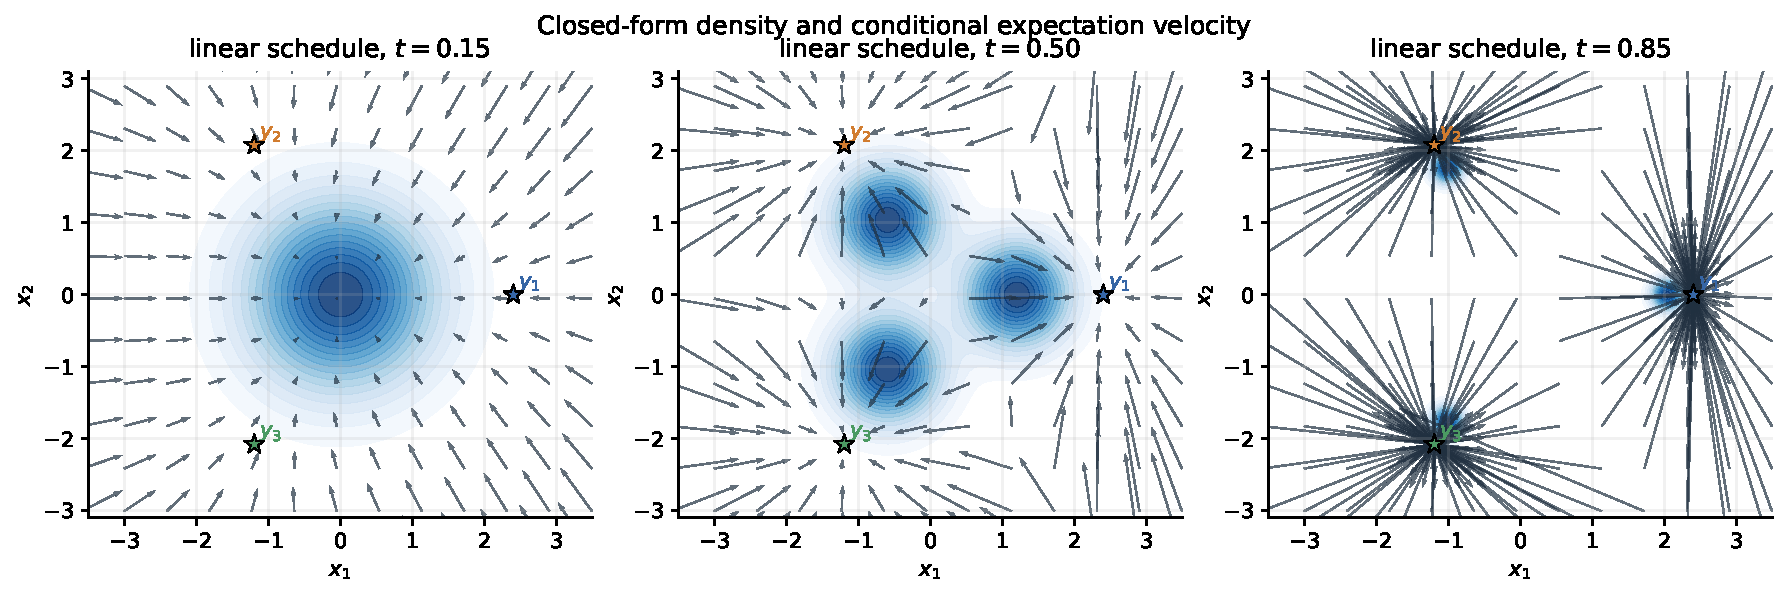
\includegraphics[width=\textwidth]{dirac_density_velocity.pdf}
\caption{Exact density contours and conditional expectation velocity for the
linear schedule.  The density is the closed-form mixture
\eqref{eq:dirac-density}; arrows show the PyTorch evaluation of
\eqref{eq:dirac-velocity}.}
\label{fig:dirac-density}
\end{figure}

\subsection{Probability-flow trajectories}

Figure~\ref{fig:dirac-trajectories} shows trajectories of the probability-flow
ODE.  Each curve is colored by the nearest Dirac mass at the final numerical
time.  The schedules share the same endpoint constraints but visibly change
the geometry of the paths.  Linear interpolation removes source variance
quickly, while the variance-preserving and cosine schedules keep broader
intermediate clouds and produce different bending before the terminal collapse.

\begin{figure}[t]
\centering
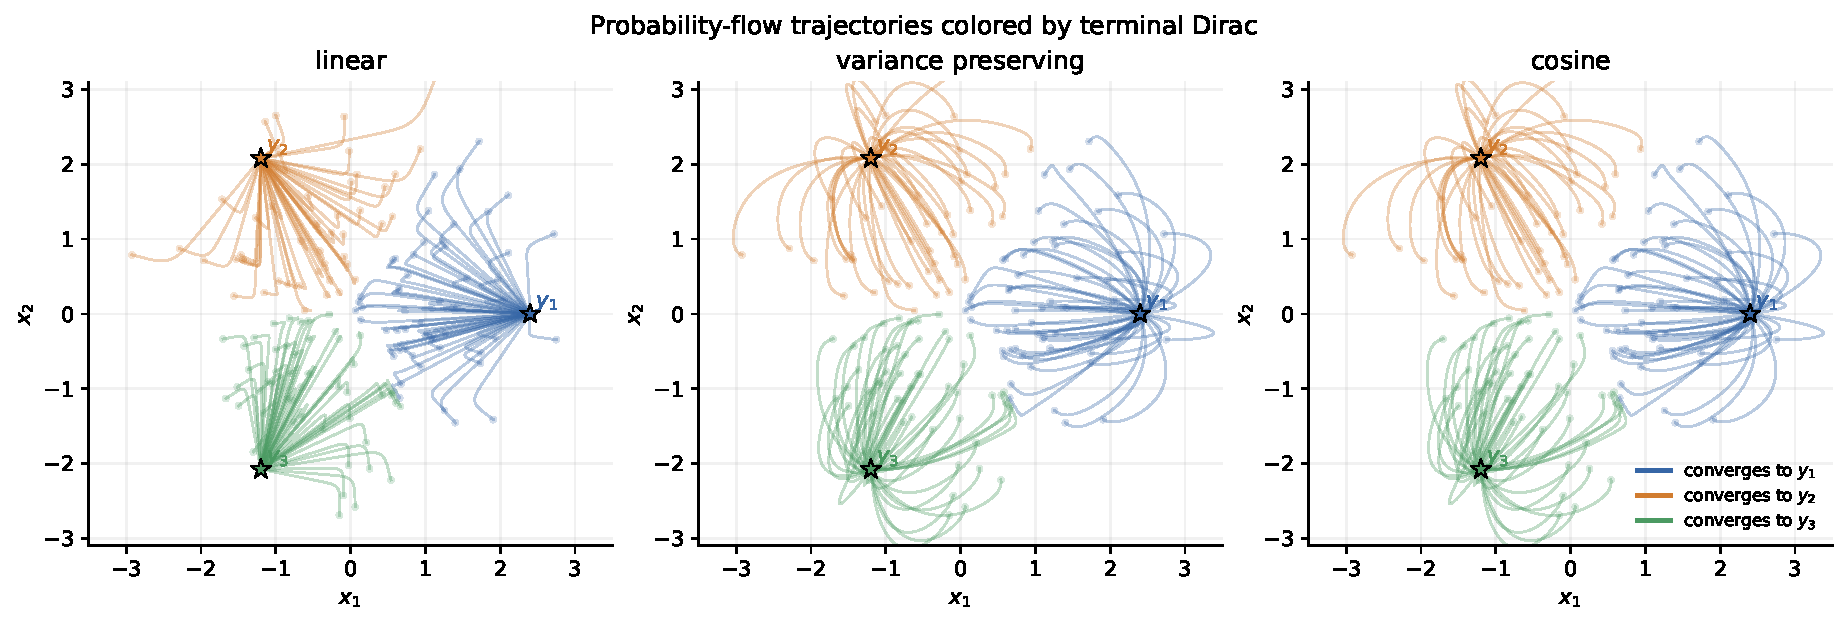
\includegraphics[width=\textwidth]{dirac_schedule_comparison.pdf}
\caption{Sample trajectories of the flow-matching ODE for three schedules.
Colors indicate the Dirac mass to which the final point is closest.}
\label{fig:dirac-trajectories}
\end{figure}

\subsection{Comparison with semi-discrete optimal transport}

Because the target points form an equilateral triangle and the source Gaussian
is rotationally invariant, the equal-mass semi-discrete OT Laguerre cells have
equal dual weights.  Since the three targets have the same norm, those cells
are exactly the nearest-vertex cones.  The OT map is therefore
\[
        T_{\rm OT}(x)=y_{\arg\min_k \|x-y_k\|},
\]
up to cell boundaries of zero Gaussian measure.  Its displacement
interpolation follows straight rays,
\[
        x_t=(1-t)x+tT_{\rm OT}(x).
\]
Figure~\ref{fig:ot-rays} contrasts these rays with the conditional-expectation
flows.  Both constructions connect the same endpoint measures, but the
stochastic-interpolant flow is selected by the coupling and schedule, not by
the quadratic transport cost.

\begin{figure}[t]
\centering
\begin{subfigure}{0.47\textwidth}
\centering
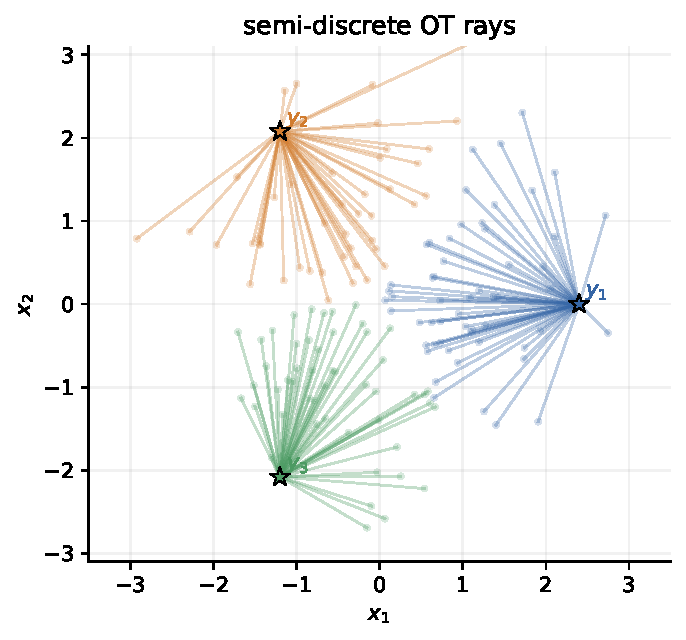
\includegraphics[width=\textwidth]{dirac_ot_trajectories.pdf}
\caption{Semi-discrete OT rays.}
\end{subfigure}
\hfill
\begin{subfigure}{0.47\textwidth}
\centering
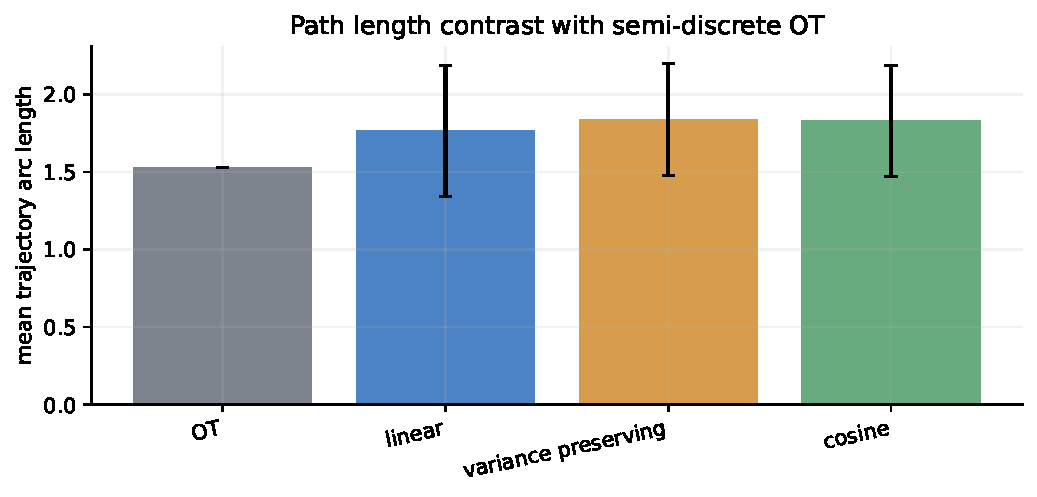
\includegraphics[width=\textwidth]{dirac_path_length_comparison.pdf}
\caption{Mean trajectory arc length.}
\end{subfigure}
\caption{The symmetric OT map partitions the source by nearest target point and
moves along straight segments.  The flow-matching trajectories are generally
curved and have schedule-dependent arc length.}
\label{fig:ot-rays}
\end{figure}

\section{Gaussian Endpoint Geometry}

We now take independent Gaussian endpoints
\[
        X_0\sim\mathcal N(0,\Sigma_0),\qquad
        X_1\sim\mathcal N(0,\Sigma_1),
\]
where \(\Sigma_0,\Sigma_1\) are symmetric positive definite matrices.

\begin{theorem}[Gaussian stochastic-interpolant flow]
\label{thm:gaussian-flow}
Let \(X_t=a(t)X_0+b(t)X_1\) with independent centered Gaussian endpoints.
Define
\[
        \Sigma_t=a(t)^2\Sigma_0+b(t)^2\Sigma_1,\qquad
        A=\Sigma_0^{-1/2}\Sigma_1\Sigma_0^{-1/2},
\]
and
\[
        M_t=a(t)^2I+b(t)^2A .
\]
Then \(X_t\sim\mathcal N(0,\Sigma_t)\), and the conditional velocity is linear,
\begin{equation}
        u_t(x)=B_tx,\qquad
        B_t=(a(t)\dot a(t)\Sigma_0+b(t)\dot b(t)\Sigma_1)\Sigma_t^{-1}.
        \label{eq:gaussian-velocity}
\end{equation}
The flow map from time \(0\) to time \(t\) is
\begin{equation}
        T_t=\Sigma_0^{1/2}M_t^{1/2}\Sigma_0^{-1/2}.
        \label{eq:gaussian-map}
\end{equation}
In particular, if \(a(1)=0\) and \(b(1)=1\),
\begin{equation}
        T_1=\Sigma_0^{1/2}
        \left(\Sigma_0^{-1/2}\Sigma_1\Sigma_0^{-1/2}\right)^{1/2}
        \Sigma_0^{-1/2}.
        \label{eq:terminal-si-map}
\end{equation}
The Gaussian optimal-transport map is
\begin{equation}
        T_{\rm OT}=
        \Sigma_0^{-1/2}
        \left(\Sigma_0^{1/2}\Sigma_1\Sigma_0^{1/2}\right)^{1/2}
        \Sigma_0^{-1/2}.
        \label{eq:gaussian-ot-map}
\end{equation}
Moreover, \(T_1=T_{\rm OT}\) if and only if
\(\Sigma_0\Sigma_1=\Sigma_1\Sigma_0\).
\end{theorem}

\begin{proof}
The covariance formula follows from independence:
\[
        \Cov(X_t)=a(t)^2\Sigma_0+b(t)^2\Sigma_1.
\]
For a joint centered Gaussian vector, conditional expectation is linear.
Since
\[
        \Cov(X_0,X_t)=a(t)\Sigma_0,\qquad
        \Cov(X_1,X_t)=b(t)\Sigma_1,
\]
we have
\[
        \mathbb E[X_0\mid X_t=x]
        =a(t)\Sigma_0\Sigma_t^{-1}x,\qquad
        \mathbb E[X_1\mid X_t=x]
        =b(t)\Sigma_1\Sigma_t^{-1}x.
\]
Substituting into \eqref{eq:conditional-velocity} gives
\eqref{eq:gaussian-velocity}.

It remains to verify the flow map.  Write
\[
        \Sigma_t=\Sigma_0^{1/2}M_t\Sigma_0^{1/2},
\]
where \(M_t=a(t)^2I+b(t)^2A\).  Since \(M_t\) and
\(\dot M_t=2a(t)\dot a(t)I+2b(t)\dot b(t)A\) are polynomials in \(A\), they
commute.  Therefore
\[
        \frac{d}{dt}M_t^{1/2}
        =\frac12\dot M_t M_t^{-1/2}.
\]
Differentiating \eqref{eq:gaussian-map} yields
\[
        \dot T_tT_t^{-1}
        =\Sigma_0^{1/2}
        \frac12\dot M_tM_t^{-1}
        \Sigma_0^{-1/2}
        =(a\dot a\,\Sigma_0+b\dot b\,\Sigma_1)\Sigma_t^{-1}
        =B_t .
\]
Also \(T_0=I\), so \(T_t\) is the linear flow generated by \(B_t\).  The
endpoint formula \eqref{eq:terminal-si-map} follows by setting \(t=1\).

Formula \eqref{eq:gaussian-ot-map} is the classical Brenier map between
centered Gaussians.  It is symmetric positive definite.  The map
\eqref{eq:terminal-si-map} also sends \(\Sigma_0\) to \(\Sigma_1\), but it is
the Brenier map exactly when it is symmetric.  Symmetry of
\(T_1=\Sigma_0^{1/2}A^{1/2}\Sigma_0^{-1/2}\) is equivalent to
\(\Sigma_0 A^{1/2}=A^{1/2}\Sigma_0\), hence to
\(\Sigma_0 A=A\Sigma_0\).  In an eigenbasis of \(\Sigma_0\), this condition is
equivalent to \(\Sigma_1\) being block diagonal on the eigenspaces of
\(\Sigma_0\), which is exactly \(\Sigma_0\Sigma_1=\Sigma_1\Sigma_0\).  In that
commuting case the matrices are simultaneously diagonalizable and the two maps
both reduce to multiplication by
\(\diag(\sqrt{\lambda_{1,i}/\lambda_{0,i}})\).
\end{proof}

\subsection{Numerical covariance display}

The notebook \texttt{python/gaussian\_covariance\_ellipses.ipynb} plots the
ellipses of \(\Sigma_t\) for a noncommuting pair
\((\Sigma_0,\Sigma_1)\).  Figure~\ref{fig:gaussian-ellipses} shows that the
choice of \(a,b\) changes the covariance path, even though every schedule has
the same endpoints.  Figure~\ref{fig:gaussian-maps} displays the endpoint map
from \eqref{eq:terminal-si-map} and the Brenier map from
\eqref{eq:gaussian-ot-map}; both match the target covariance, but the maps are
different because the covariances do not commute.

\begin{figure}[t]
\centering
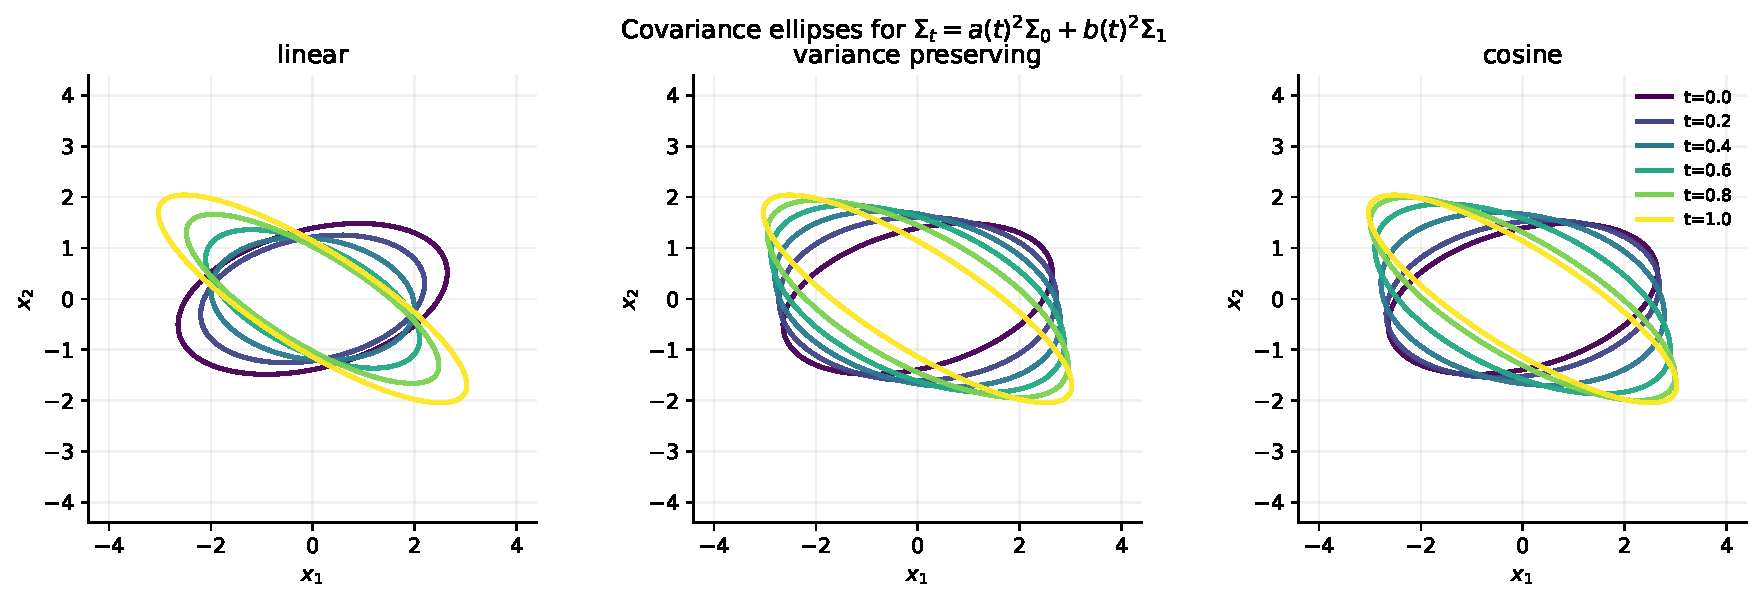
\includegraphics[width=\textwidth]{gaussian_covariance_ellipses.pdf}
\caption{Covariance ellipses for the Gaussian stochastic interpolant under the
three schedules.  The endpoint ellipses are common; the intermediate covariance
geometry is schedule-dependent.}
\label{fig:gaussian-ellipses}
\end{figure}

\begin{figure}[t]
\centering
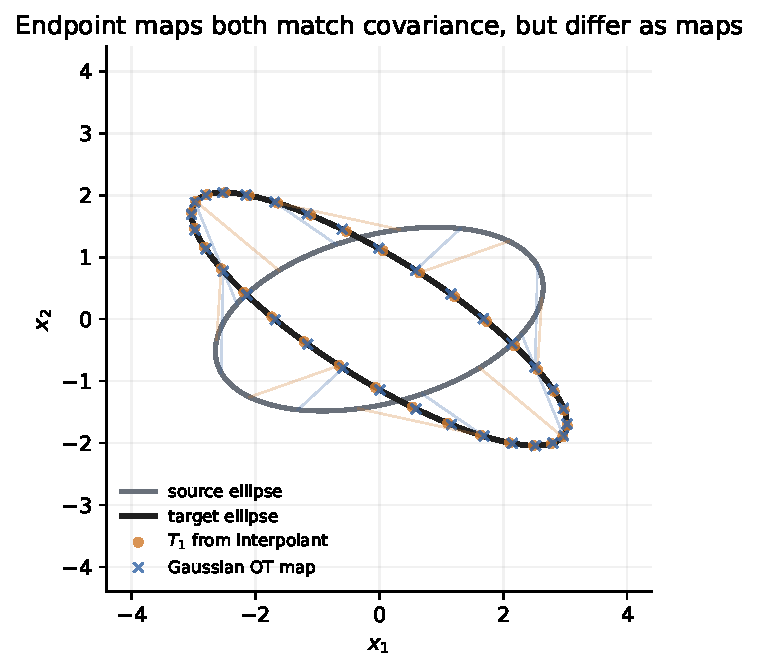
\includegraphics[width=0.62\textwidth]{gaussian_endpoint_maps.pdf}
\caption{For noncommuting covariances, the stochastic-interpolant endpoint map
\(T_1\) and the Gaussian OT map both push \(\Sigma_0\) to \(\Sigma_1\), but
they differ as linear maps.}
\label{fig:gaussian-maps}
\end{figure}

\section{Discussion}

These examples separate three objects that are sometimes conflated: the
marginal path \(\rho_t\), the deterministic flow that realizes that marginal
path, and the OT map selected by the quadratic cost.  A stochastic interpolant
fixes a coupling and schedule, then obtains a velocity by conditional
expectation.  This velocity is easy to compute in the examples above, and it is
the target of the flow-matching regression in data-driven settings.  However,
unless the coupling and geometry are specially aligned, the terminal
probability-flow map is not the Brenier OT map.

The Gaussian theorem makes this conclusion algebraic.  Even when both endpoint
distributions are Gaussian and the full flow is linear, the independent
endpoint interpolant produces \(T_1=\Sigma_0^{1/2}
(\Sigma_0^{-1/2}\Sigma_1\Sigma_0^{-1/2})^{1/2}\Sigma_0^{-1/2}\), whereas OT
requires the symmetric positive map.  Equality occurs exactly in the commuting
case, where the covariance matrices share eigenspaces and all relevant
matrices are simultaneously diagonal.

\bibliographystyle{plainnat}
\bibliography{references}

\end{document}
